\documentclass{article}
\usepackage{qilin}
\tikzstyle{process} = [rectangle, rounded corners, minimum width=1.5cm, minimum height=0.5cm,align=center, draw=black, fill=gray!30, auto]
\title{Knot Theory}
\author{QiLin Xue}
\date{Fall 2021}
\usepackage{mathrsfs}
\usetikzlibrary{arrows}
\usepackage{stmaryrd}
\usepackage{accents}
\newcommand{\ubar}[1]{\underaccent{\bar}{#1}}
\usepackage{1350}
\usepackage{tikz}
\usetikzlibrary{knots} 
\usepgfmodule{decorations}
\usepackage{mmacells}
\mmaDefineMathReplacement[⧴]{:>}{:\hspace{-.2em}\to}[2]


\begin{document}

\maketitle
\tableofcontents

\newpage
\section{Introduction to Knots: Reidemeister moves, 3-colourings}
Knot theory is the study of knots. Specifically, we are interested in answering questions about the properties of knots and whether two knots are equivalent, i.e. can we deform the left knot (the \emf{trefoil}) to get to the right knot (the \emf{unknot})?
\begin{center}
    \hspace{-10mm}
    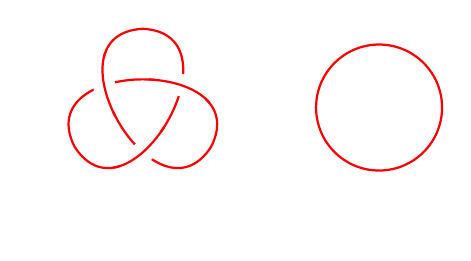
\begin{tikzpicture}
        \begin{knot}[
            clip width=10,
            consider self intersections
        ]
            \strand[red,thick] (90:1)
                \foreach \x in {1,2,3} {
                    to [bend left=117,looseness=1.9] ({90+120*\x}:1)
                }
            ;
            \flipcrossings{1,3}
            \strand[red,thick] (3,0) circle[radius=0.8];
        \end{knot}
    \end{tikzpicture}
\end{center}\vspace{-6mm}
Why do we care? Apart from being a party trick, knot theory has applications in topology, combinatorics, homological algebra, representation theory, algebraic topology, differential geometry, quantum field theory, computer algebra, and more.

It turns out the above two knots are not equivalent. While it may be easy to see so intuitively, it's not always the case. For example, the \emf{Perko Pair}
\begin{center}
    \includegraphics[width=0.3\linewidth]{figures/perko.png}
\end{center}
were thought to be distinct for a very long time, but they are actually equivalent. We will define a knot very loosely using combinatorics:
\begin{definition}
    A knot can be represented by a quadrivalent graph (with the exception of the unknot) using a knot diagram, such as the ones illustrated above. 
\end{definition}
The reason we don't give the formal definition is that it uses topological maps (and there are multiple equivalent definitions), which causes it to get very ugly fast. We will revisit this formal definition in a later section.
\subsection{Reidemeister Moves}
The Reidemeister moves are a set of moves that can be applied to a knot to make it equivalent to another knot. The moves are defined as follows:
\begin{center}
    \includegraphics[width=0.4\linewidth]{figures/reidemeister.jpg}
\end{center}
The first Reidemeister move, $R1$ tells us that we can untwist a \emf{kink}. The second $R2$ talks about poking/unpoking, and the third talks about sliding.

We will state (but not yet prove) the following properties of the Reidemeister moves:
\begin{theorem}
    The set of knots is equivalent to the set of knot diagrams modulo the Reidemeister moves.
    \begin{equation}
        \{\text{knots}\} = \frac{\{\text{knot diagrams}\}}{\{\text{Reidemeister moves}\}}
    \end{equation}
\end{theorem}
To prove that two knots are equivalent, we need to find a sequence Reidemeister moves to transform one knot into the other. However, this can often be tricky (since there can be an infinite combination of moves) so if two knots are different, we cannot show they are different by ``failing'' to find a sequence of moves.

As a result, we will need another tool, known as \emf{invariants.}
\subsection{3-Colouring Knot Invariant}
\begin{definition}
    A function on the set of knot diagrams with values that are easily computable (i.e. with values in $\mathbb{Z}$, polynomials, matrices, etc.) and that does not change if you perform $R$-moves are known as \emf{invariants.}
\end{definition}
There are several knot invariants but we will only consider the number of \emf{3-colourings} of the knot.
\begin{definition}
    A 3-colouring is an assignment of colours $\{R,G,B\}$ to the arcs of the knot. A \emf{legit} 3-colouring is when only $1$ or $3$ colours are used. We will let $\lambda$ denote the number of legit 3-colourings.
\end{definition}
For example, the following is an example of a 3-colouring. Note that not every colour needs to be used.
\begin{center}
    \includegraphics[width=0.2\linewidth]{figures/trefoil_3color.png}
\end{center}
\begin{theorem}
        The number of 3-colourings of a knot is an invariant.
\end{theorem}
\begin{proof}
    We simply need to establish a bijection between the number of legit 3-colourings in the left hand and right hand sides of the Reidemeister moves.
    \begin{center}
        \includegraphics[width=0.4\linewidth]{figures/reidemeister_3coloring.png}
    \end{center}
    \vspace{-6mm}
\end{proof}
\begin{example}
    Let us compare the trefoil knot to the unknot. There are three arcs in the trefoil knot. It turns out that the color of the third arc is completely determined by the color of the first two arcs, which are independent to each other.
    \vspace{2mm}

    On the other hand, the unknot only has three legit 3-colourings. Therefore $\lambda(\text{trefoil}) = 9$, $\lambda(\text{unknot}) = 3$, so these two knots are not equivalent.
\end{example}
\section{The Kauffman Bracket}
There are two annoying issues with the 3-colouring knot invariant. If $D$ is a knot diagram:
\begin{itemize}
    \item $\lambda(D)$ is often $3$ or $9$ (and occasionally $27$) for simple knots. This means that oftentimes, different knots will have the same $\lambda$.
    \item If the knot is very complex, it may be very difficult to compute $\lambda(D).$
\end{itemize}
Therefore, we wish to find a better way of doing things.
\begin{definition}
    We introduce the \emf{Kauffman bracket} $\langle D\rangle$ from two axioms:
    \begin{enumerate}
        %the first rule
        \item $\left\langle\KPA \sqcup D \right\rangle=d\langle D\rangle$
        
        \item $\left\langle\KPB\right\rangle=
        A\left\langle\KPD\right\rangle + B \left\langle \KPC \right\rangle$
    \end{enumerate}
    where $\left\langle\KPD\right\rangle$ is known as the \emf{0-smoothing} and $\left\langle \KPC\right\rangle$ is known as the \emf{1-smoothing}. We can imagine the ends of the bracket as being the two ends of the knot (where the bottom two vertices of each diagram are connected.)
\end{definition}
For example, consider a \emf{link} (which we will not precisely define), known as the \emf{Hopf Link}:
\begin{center}
    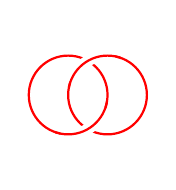
\begin{tikzpicture}[scale=0.5]
        \begin{knot}[
            clip width=5,
            flip crossing={1},
            ]
            \strand [thick, red  ] (1.5,0) circle (1.0cm);
            \strand [thick, red ] (2.5,0) circle (1.0cm);
        \end{knot}
    \end{tikzpicture}
\end{center}
We can apply two successive smoothings to this link to get the following (ignore the mapping names):
\begin{center}
    \includegraphics[width=0.5\linewidth]{figures/hopf_link_bracket.png}
\end{center}
so
\begin{align}
    \langle H\rangle &= A^2\langle H_4\rangle + AB\langle H_3\rangle + AB\langle H_2\rangle + B^2 \langle H_1\rangle \\ 
    &= A^2d^2 + 2ABd + B^2d^2
\end{align}
\begin{theorem}
    Let $B=A^{-1}$ and let $d=-A^2-A^{-2}.$ Then $\langle D\rangle$ is an invariant for $R2$ and $R3$.
\end{theorem}
\begin{proof}
    We want to show that the $R2$ move is invariant. To do so, we simple compute it in a similar way above, and we get a system of two equations:
    \begin{align}
        AB &= 1 \\ 
        A^2+B^2 + ABd &= 1
    \end{align}
    which after solving gives the necessary conditions in the theorem. Then, using these relationships, we can show that the $R3$ move is invariant also. It may seem difficult to compute as there are now three crossings, but after simplifying a single crossing, we can relate it back to the $R2$ case which we have solved.
\end{proof}
However, if we try to compute $R1$, it turns out that
\begin{equation}
    \left\langle \kinkA \right\rangle = (-A^3) \left\langle \lineknot\right \rangle
\end{equation}
so it seems like $\langle D\rangle$ is not an invariant in general. However, as with many other concepts in knot theory, if something doesn't behave as expected for $R1$, there are often ways to circumvent it. The idea is that there are variants of the $R1$ move. For example, we have
\begin{equation}
    \left\langle \kinkB \right\rangle = (-A^{-3}) \left\langle \lineknot\right \rangle
\end{equation}
Using this, we can define the \emf{writhe} of a knot diagram as
\begin{definition}
    The writhe $w$ is defined as
    \begin{equation}
        w(D) = \sum_\text{crossings $x\in D$} \text{sign}(x)
    \end{equation} 
    where crossings now have orientations. We define them such that
    \begin{center}
        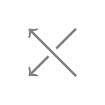
\begin{tikzpicture}
            \draw[color=gray,thick,<-] (-0.3,0.3) -- (0.3,-0.3);
            \draw[color=gray,thick,<-] (-0.3,-0.3) -- (-0.05,-0.05);
            \draw[color=gray,thick] (0.05,0.05) -- (0.3,0.3);
        \end{tikzpicture}
    \end{center}
    has positive sign and
    \begin{center}
        
\begin{tikzpicture}
            \draw[color=gray,thick,<-] (-0.3,0.3) -- (0.3,-0.3);
            \draw[color=gray,thick] (-0.3,-0.3) -- (-0.05,-0.05);
            \draw[color=gray,thick,->] (0.05,0.05) -- (0.3,0.3);
        \end{tikzpicture}
    \end{center}
    has negative sign. We can remember using the \emf{right-hand rule.} Point your thumb towards the direction of one arrow and curl your fingers. If your fingers point in the direction of the other arrow, then its positive. Otherwise, its negative. 
\end{definition}
\begin{theorem}
    The writhe of a knot diagram is invariant under the $R2$ and $R3$ moves.
\end{theorem}
\begin{proof}
    We can show that the writhe is not affected by $R2$ and $R3$ moves by showing that for any arrows we draw, the writhe of the left hand and the right hand side are the same. In fact, this should be very easy to see even without drawing arrows.
\end{proof}
We now have two quantities that are \textit{almost} invariants. We will see in the next section how we can combine these two quantities to get an actual \textit{invariant} that will be more helpful.

\newpage
\section{The Jones Polynomial}
We wish to add a factor such that it counts the number of kinks (and their orientations) such that when $\langle K\rangle$ has a factor of $(-A^{\pm 3})$, this factor has a factor of $(-A^{\mp 3})$. This is called the \emf{Jones Polynomial}.
\begin{theorem}
    The Jones Polynomial is an invariant. Let $K$ be a knot diagram. Then,
    \begin{equation}
        J(K) = (-A^3)^{-w(K)} \frac{\langle K\rangle}{d}
    \end{equation}
    where the $d$ comes from the fact that the numerator will always be divisible by $d$. The Jones Polynomial is a Laurent Polynomial.
\end{theorem}
It also turns out that factors of $A$ are a power of $4$, so we often make the substitution $A \to q^{-4}$. This leads to the Jones-Skein Relation 
\begin{theorem}
    The \emf{Jones-Skein Relation} is another way of computing the Jones Polynomial. 
    \begin{equation}
        q^{-1}J\left(\upcross\right)-qJ\left(\downcross\right) = (q^{1/2}-q^{-1/2})J\left(\KPDArrow\right)
    \end{equation}
    The idea is that every knot can be undone by flipping \emf{overcrossings} to \emf{undercrossings}, and the other way around.
\end{theorem}
We can change any knot into the unknot through a \emf{descending knot diagram.} For example, suppose we have the trefoil (left). We can change it into the unknot by flipping over one of the crossings such that the knot is always descending if we start from the top and move to the left. Therefore, we can imagine the right hand side as a projection.
\begin{center}
    \hspace{-10mm}
    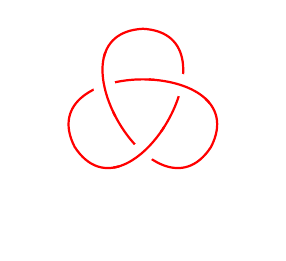
\begin{tikzpicture}
        \begin{knot}[
            clip width=10,
            consider self intersections
        ]
            \strand[red,thick] (90:1)
                \foreach \x in {1,2,3} {
                    to [bend left=117,looseness=1.9] ({90+120*\x}:1)
                }
            ;
            \flipcrossings{1, 3}
        \end{knot}
    \end{tikzpicture}
    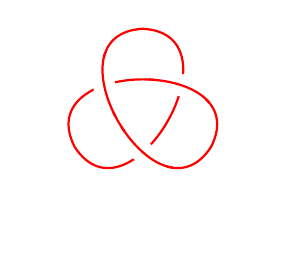
\begin{tikzpicture}
        \begin{knot}[
            clip width=10,
            consider self intersections
        ]
            \strand[red,thick] (90:1)
                \foreach \x in {1,2,3} {
                    to [bend left=117,looseness=1.9] ({90+120*\x}:1)
                }
            ;
            \flipcrossings{1,2,3}
        \end{knot}
    \end{tikzpicture}
\end{center}\vspace{-6mm}
Therefore, the Jones-Skein essentially tells us the ``cost'' of changing a crossing, i.e. there is a price to pay for changing a link into the disjoint union of unknots. This means we need to show that
\begin{equation}
    J\left(\KPA^k\right)=(-q^{1/2}-q^{-1/2})^k
\end{equation}
\subsection{PD-Notation}
We go through a few definitions: An \emf{arc} goes undercrossings to undercrossings while an \emf{edge} goes from a crossing to a crossing. We can label the edges by starting at an arbitrary location and moving along it in one direction.
\begin{center}
    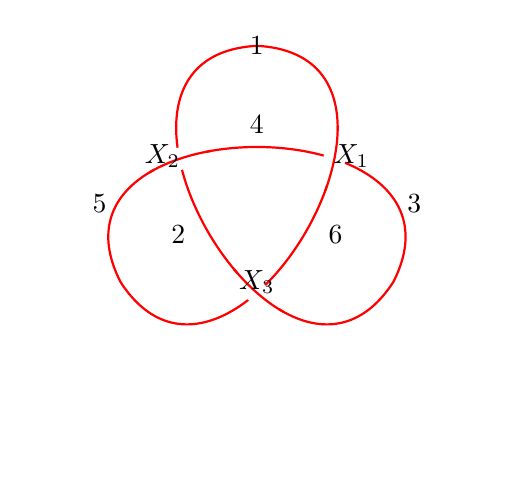
\begin{tikzpicture}[scale=2]
        \begin{knot}[
            clip width=10,
            consider self intersections,
        ]
            \strand[red,thick] (90:1)
                \foreach \x in {1,2,3} {
                    to [bend left=117,looseness=1.9] ({90+120*\x}:1)
                }
            ;
            \flipcrossings{2}
        \end{knot}

        % Add label at (0,1)
        \node[] at (0,1) {$1$};
        \node[] at (-0.5,-0.2) {$2$};
        \node[] at (1,0) {$3$};
        \node[] at (0,0.5) {$4$};
        \node[] at (-1,0) {$5$};
        \node[] at (0.5, -0.2) {$6$};

        \node[] at (0.6, 0.3) {$X_1$};
        \node[] at (-0.6, 0.3) {$X_2$};
        \node[] at (0, -0.5) {$X_3$};

    \end{tikzpicture}
\end{center}\vspace{-6mm}
We can label crossings by the four edges it is composed of. For example,
\begin{center}
    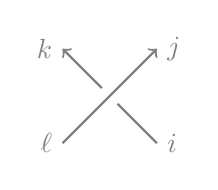
\begin{tikzpicture}
        \draw[color=gray,thick,->] (-0.6,-0.6) node[left] {$\ell$} -- (0.6,0.6) node[right] {$j$};
        \draw[color=gray,thick] (0.6,-0.6) node[right] {$i$} -- (0.1,-0.1);
        \draw[color=gray,thick,->] (-0.1,0.1) -- (-0.6,0.6) node[left] {$k$};
    \end{tikzpicture}
\end{center}
would be named $X_{ijk\ell}.$ If we label the crossings of the trefoil, we will have 
\begin{equation}
    X^+_{3146}\quad\quad X^+_{1524}\quad\quad X^+_{5362}
\end{equation}
Remember that we start from edge $1$ and travel counterclockwise. The $+$ exponent denotes that these crossings are positive.
\begin{theorem}
    This list of crossing information determines $D$ as a diagram on $S^2.$
\end{theorem}
The proof is left as an exercise.

Similarly, when we apply smoothings to a crossing, we can label the corresponding edges by the two edges that are involved. For example applying the 0-smoothing and 1-smoothing,
\begin{center}
    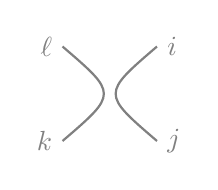
\begin{tikzpicture}[scale=2]
        \draw[color=gray,thick] (-0.3,-0.3) node[left]{$k$} .. controls (0.05,0) .. (-0.3,0.3) node[left] {$\ell$};
        \draw[color=gray,thick] (0.3,-0.3) node[right] {$j$} .. controls (-0.05,0) .. (0.3,0.3) node[right] {$i$};
    \end{tikzpicture}
    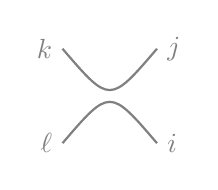
\begin{tikzpicture}[scale=2]
        \draw[color=gray,thick,] (-0.3,0.3) node[left] {$k$} .. controls (0,-0.05) .. (0.3,0.3) node[right] {$j$};
        \draw[color=gray,thick,] (-0.3,-0.3) node[left] {$\ell$}.. controls (0,0.05) .. (0.3,-0.3) node[right] {$i$};
    \end{tikzpicture}
\end{center}
we can label the edges as $P_{k\ell},P_{ij},P_{jk},P_{i\ell}$. We can treat this as an imaginary vertex in the middle of each edge, and these are ``names'' of each \emf{vertex}.
\subsection{Applying it with Mathematica}
We can define a trefoil knot diagram using
\begin{mmaCell}{Input}
    K = PD[Xp[3, 1, 4, 6], Xp[1, 5, 2, 5], Xp[5, 3, 6, 2]] 
\end{mmaCell}
We want to apply a rule
\begin{mmaCell}{Input}
    t1 = K /. {Xp[i_, j_, k_, l_] :> Ap[i, j] * p[k, l] + \mmaSup{A}{-1}p[i, l] * p[j, k]}
\end{mmaCell}
\begin{mmaCell}{Output}
    PD[\mmaFrac{p[1,4]*p[3,6]}{A}+Ap[3,1]*p[4,6],Ap[1,5]*p[2,4]+\mmaFrac{p[1,4]*p[5,2]}{A},\mmaFrac{p[3,6]*p[5,2]}{A}+Ap[5,3]*p[6,2]]
\end{mmaCell}
which is a rule that tells us how to apply smoothings to a crossing. Each of the two terms refer to one of the two possible smoothings (for a given crossing).

However, there are really $8$ smoothings to the trefoil. Each of these smoothings is obtained by choosing a single term in the three possible expressions above, i.e. this motivates us to apply the distributive property:
\begin{mmaCell}{Input}
    Times @@ t1
\end{mmaCell}
\begin{mmaCell}{Output}
    (\mmaFrac{p[1,4]*p[3,6]}{A}+Ap[3,1]*p[4,6])(Ap[1,5]*p[2,4]+\mmaFrac{p[1,4]*p[5,2]}{A})(\mmaFrac{p[3,6]*p[5,2]}{A}+Ap[5,3]*p[6,2])
\end{mmaCell}
and calling
\begin{mmaCell}{Input}
    t2 = Expand[Times @@ t1]
\end{mmaCell}
gives us the sum of eight terms, each of which refers to a given smoothing. However this is messy (such that I won't write it out), but we can apply clever techniques to simplify it. For example,
\begin{mmaCell}{Input}
    t3 = t2 //. {p[i_, j_] * p[j_, k_] :> p[i, k]}
\end{mmaCell}
which turns two edges joined together into one long edge. This longer edge could possibly be a loop, i.e. the unknot. Therefore, we can simplify it further by replacing this with $d=-A^2-A^{-2}.$
\begin{mmaCell}{Input}
    t4 = t3 /. {p[i_, i_] :> (-\mmaSup{-A}{2}-\mmaSup{A}{-2}), \mmaSup{p[i_,j_]}{2} :> (-\mmaSup{A}{2}-\mmaSup{-A}{-2})}
\end{mmaCell}
and simplifying it gives
\begin{mmaCell}{Input}
    Expand[t4]
\end{mmaCell}
\begin{mmaCell}{Output}
    -\mmaFrac{1}{\mmaSup{A}{9}} + \mmaFrac{1}{A} + \mmaSup{A}{3} + \mmaSup{A}{7}
\end{mmaCell}
which gives the Kauffman Bracket of the trefoil.
\end{document}